
\section{Closure Test of Templates in MC}
\label{sec:mc}

The above procedure is applied to MC to test its effectiveness under `ideal' conditions. 
In order to test the 
results obtained in section \ref{sec:tempcompresults}, 
%dependence of the method on the sample composition, 
we construct templates separately from PhotonJet MC and QCD MC.
%Templates are derived from PhotonJet MC, and 
These templates are then used to predict the MET distribution in ZJets MC. The 
MC samples used are:

\begin{itemize}
\item PhotonJet MC
  \begin{itemize}
  \item \verb=/G_Pt_15to30_TuneZ2_7TeV_pythia6/Spring11-PU_S1_START311_V1G1-v1/AODSIM  =
  \item \verb=/G_Pt_30to50_TuneZ2_7TeV_pythia6/Spring11-PU_S1_START311_V1G1-v1/AODSIM  =
  \item \verb=/G_Pt_50to80_TuneZ2_7TeV_pythia6/Spring11-PU_S1_START311_V1G1-v1/AODSIM  =
  \item \verb=/G_Pt_80to120_TuneZ2_7TeV_pythia6/Spring11-PU_S1_START311_V1G1-v1/AODSIM =
  \item \verb=/G_Pt_120to170_TuneZ2_7TeV_pythia6/Spring11-PU_S1_START311_V1G1-v1/AODSIM=
  \item \verb=/G_Pt_170to300_TuneZ2_7TeV_pythia6/Spring11-PU_S1_START311_V1G1-v1/AODSIM= 	  
  \end{itemize}
\item QCD MC
  \begin{itemize}
  \item \verb=/QCD_Pt_15to30_TuneZ2_7TeV_pythia6/Spring11-PU_S1_START311_V1G1-v1/AODSIM  =
  \item \verb=/QCD_Pt_30to50_TuneZ2_7TeV_pythia6/Spring11-PU_S1_START311_V1G1-v1/AODSIM  =
  \item \verb=/QCD_Pt_50to80_TuneZ2_7TeV_pythia6/Spring11-PU_S1_START311_V1G1-v1/AODSIM  =
  \item \verb=/QCD_Pt_80to120_TuneZ2_7TeV_pythia6/Spring11-PU_S1_START311_V1G1-v1/AODSIM =
  \item \verb=/QCD_Pt_120to170_TuneZ2_7TeV_pythia6/Spring11-PU_S1_START311_V1G1-v1/AODSIM= 
  \item \verb=/QCD_Pt_170to300_TuneZ2_7TeV_pythia6/Spring11-PU_S1_START311_V1G1-v1/AODSIM= 
  \end{itemize}
\item ZJet MC
  \begin{itemize}
  \item \verb=/DYToEE_M-20_CT10_TuneZ2_7TeV-powheg-pythia/Spring11-PU_S1_START311_V1G1-v1/AODSIM=
  \item \verb=/DYToMuMu_M-20_CT10_TuneZ2_7TeV-powheg-pythia/Spring11-PU_S1_START311_V1G1-v1/AODSIM=
  \item \verb=/DYToTauTau_M-20_CT10_TuneZ2_7TeV-powheg-pythia-tauola/Spring11-PU_S1_START311_V1G1-v1/AODSIM=
	%use pythia
	%\item \verb=/DYJetsToLL_TuneD6T_M-50_7TeV-madgraph-tauola/Spring11-PU_S1_START311_V1G1-v1/AODSIM=
  \end{itemize}
\end{itemize}


Good agreement between the observed and predicted MET distributions is observed for each MC sample, 
as well as between the two samples, as shown in figures \ref{fig:mcclosurepho} and \ref{fig:mcclosureqcd}. 
Note that the low equivalent luminosity of the QCD samples ($\approx$ 300/pb) explains the lack of 
statistics in the tails.

\begin{figure}[hbt]
  \begin{center}
    \resizebox{0.8\linewidth}{!}{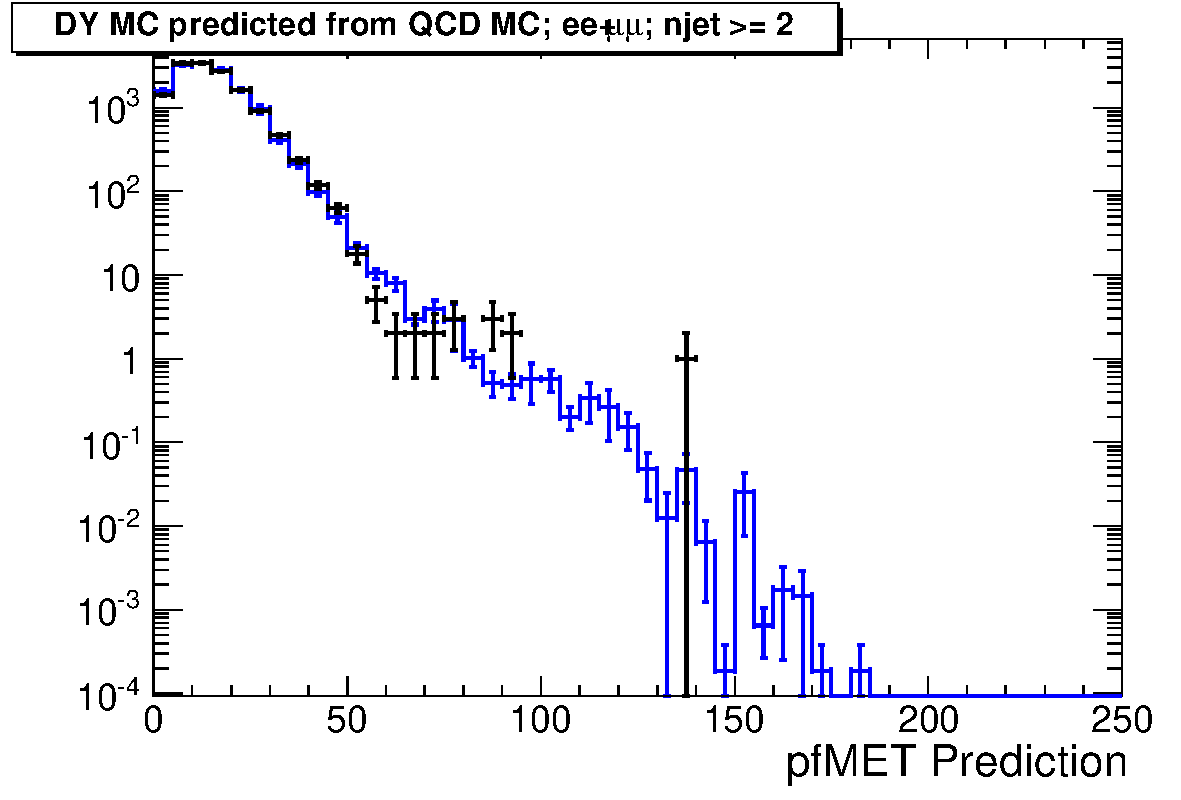
\includegraphics{plots/mcclosure_qcd.pdf}}
	\\ \medskip
    %\resizebox{\linewidth}{!}{
    \begin{tabular}{r|r|r|r|r}
      MET        & $>$ 30 GeV       & $>$ 60 GeV        & $>$ 100 GeV       & $>$ 200  \\ \hline

%tr
	  Z MC       &   921               &    15               &     1               &     0 \\
	  Prediction & 824.20 $\pm$  38.99 &  21.89 $\pm$   2.52 &   1.67 $\pm$   0.31 &   0.00 $\pm$   0.00 \\

%no tr
	  %  data    &   921               &    15               &     1               &     0 \\
	  %  pred    & 751.10 $\pm$ 101.82 &   7.78 $\pm$   0.53 &   0.45 $\pm$   0.06 &   0.00 $\pm$   0.00 \\

    \end{tabular}
	%}
	\\ \medskip
    \caption{The MET distribution in \Z plus jets MC (black) and prediction (blue) for Njet $\ge$ 2. 
	  Below the plot is tabulated the integral of the \Z plus jets MC MET and the predicted 
	  MET from QCD MC for 
	  MET $>$ 30 GeV, $>$ 60 GeV, $>$ 100 GeV, and $>$ 200 GeV. 
	}
    \label{fig:mcclosureqcd}
  \end{center}
\end{figure}


\begin{figure}[hbt]
  \begin{center}
    \resizebox{0.8\linewidth}{!}{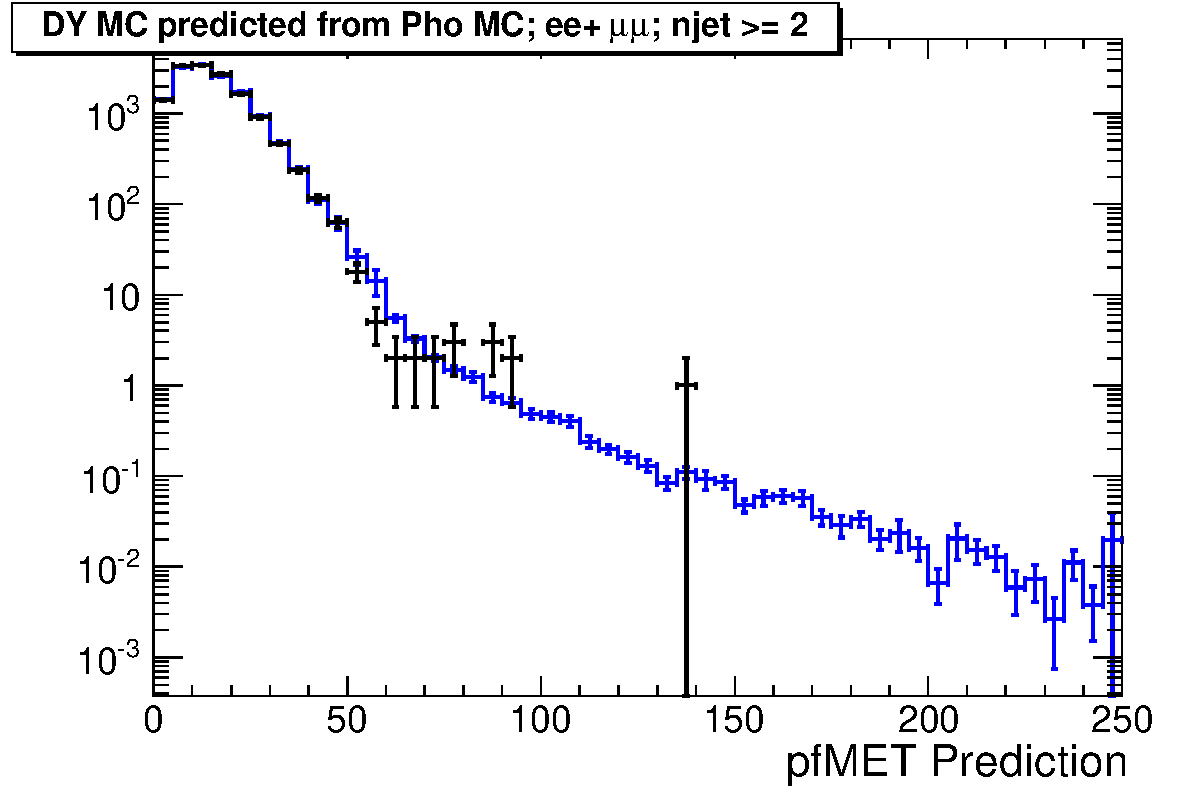
\includegraphics{plots/mcclosure_pho.pdf}}
	\\ \medskip
    %\resizebox{\linewidth}{!}{
    \begin{tabular}{r|r|r|r|r}
      MET        & $>$ 30 GeV       & $>$ 60 GeV        & $>$ 100 GeV       & $>$ 200  \\ \hline
%tr
	  Z MC       &   921               &    15               &     1               &     0 \\
	  Prediction & 959.15 $\pm$  27.00 &  19.39 $\pm$   0.58 &   2.28 $\pm$   0.09 &   0.07 $\pm$   0.01 \\
	  
%no tr
%	  Z MC       &   921               &    15               &     1               &     0 \\
%	  Prediction & 953.60 $\pm$  31.28 &  17.94 $\pm$   0.66 &   2.45 $\pm$   0.10 &   0.11 $\pm$   0.02 \\

    \end{tabular}
	%}
	\\ \medskip
    \caption{The MET distribution in \Z plus jets MC (black) and prediction (blue) for Njet $\ge$ 2. 
	  Below the plot is tabulated the integral of the \Z plus jets MC MET and the predicted 
	  MET from photon plus jets MC for 
	  MET $>$ 30 GeV, $>$ 60 GeV, $>$ 100 GeV, and $>$ 200 GeV. 
	}
    \label{fig:mcclosurepho}
  \end{center}
\end{figure}


%2010 results
%      MET                   & $>$ 30 GeV & $>$ 60 GeV  & $>$ 120 GeV \\ \hline
%      Z+jets observed         &      184   &    10       & 0          \\
%      $\gamma$+jets predicted &   182.21   &    11.52    & 1.40       \\


%\begin{wrapfigure}{r}{0.6\textwidth}
%\vspace{-25pt}
%\begin{center}
%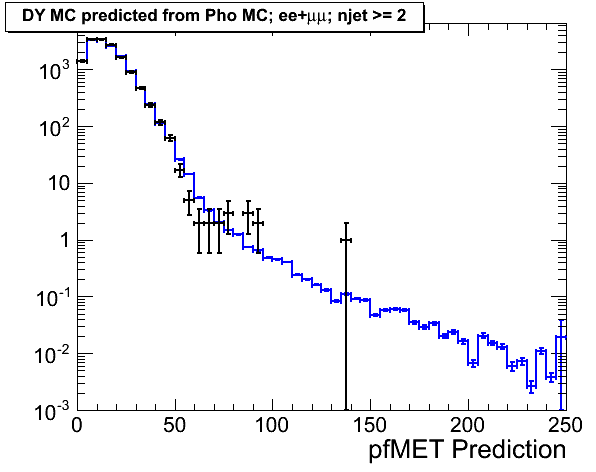
\includegraphics[width=0.8\textwidth]{plots/mcclosure}
% \caption{\label{fig:mcclosure} The MET distribution in Z+jets MC (black) and prediction (blue) for Njet $\ge$ 2. Below the plot is tabulated the integral of the observed Z+jets MC MET and the predicted MET from $\gamma$+jets MC for MET $>$ 30 GeV, $>$ 60 GeV and $>$ 120 GeV. The quantity (observed-predicted)/predicted as a function of MET is shown above the plot.}
%\end{center}
%\vspace{-20pt}
%\end{wrapfigure}
